\documentclass[11pt]{article}
\usepackage{amsthm}
\usepackage{amssymb}
\usepackage{enumitem}
\usepackage{amsmath, physics}
\usepackage{bm}
\usepackage{adjustbox}
\usepackage{mathrsfs}
\usepackage{graphicx}
\usepackage{siunitx}
\usepackage[mathscr]{euscript}

\title{\textbf{Solved selected problems of Modern Physics for Scientists and Engineers - John Taylor}}
\author{Franco Zacco}
\date{}

\addtolength{\topmargin}{-3cm}
\addtolength{\textheight}{3cm}

\newcommand{\N}{\mathbb{N}}
\newcommand{\Z}{\mathbb{Z}}
\newcommand{\Q}{\mathbb{Q}}
\newcommand{\R}{\mathbb{R}}
\newcommand{\diam}{\text{diam}}
\newcommand{\cl}{\text{cl}}
\newcommand{\bdry}{\text{bdry}}
\newcommand{\inter}{\text{int}}
\newcommand{\hatx}{\bm{\hat{x}}}
\newcommand{\haty}{\bm{\hat{y}}}
\newcommand{\hatz}{\bm{\hat{z}}}
\newcommand{\hatrho}{\bm{\hat{\rho}}}
\newcommand{\hatphi}{\bm{\hat{\phi}}}
\newcommand{\hatr}{\bm{\hat{r}}}
\newcommand{\hattheta}{\bm{\hat{\theta}}}
\newcommand{\sci}[1]{\times 10^{#1}}
\newcommand{\expect}[1]{\left\langle {#1} \right\rangle}

\theoremstyle{definition}
\newtheorem*{solution*}{Solution}
\renewcommand*{\proofname}{\bf{Solution}}

\begin{document}
\maketitle
\thispagestyle{empty}

\section*{Chapter 10 - Electron Spin}

\begin{proof}{\textbf{10.1}}
Given that the charge density is given by $\rho(r) = -e|\psi(r)|^2$, and that
the probability of finding the electron between $a_B$ and $\infty$ is $0.67$
then the enclosed charge is
\begin{align*}
    Q = \int_0^{a_B} \rho(r)~dr = -e\int_0^{a_B} |\psi(r)|^2~dr = -e(1 - 0.67)
    = -0.33e
\end{align*}
Using Gauss' law, taking a spherical Gaussian surface we see that
\begin{align*}
    \mathscr{E} \cdot 4\pi a_B^2 &= \frac{Q}{\varepsilon_0}\\
    \mathscr{E} &= \frac{-0.33e}{4\pi r^2 \varepsilon_0}\\
    \mathscr{E} &= \frac{0.33\cdot 1.602\sci{-19}}
    {4\pi \cdot (5.29\sci{-11})^2 \cdot 8.854\sci{-12}}\\
    \mathscr{E} &= 169.79\sci{9}~V/m
\end{align*}
\end{proof}

\cleardoublepage
\begin{proof}{\textbf{10.2}}
\begin{itemize}
\item [\textbf{(a)}] Given that $\rho(r) = \rho_0e^{-r/R}$ is the average
charge distribution of $Z-1$ electrons then must be that
\begin{align*}
    \int \rho(r)~dV &= Q\\
    4\pi\int_0^\infty \rho_0 e^{-r/R} r^2~ dr &= -(Z-1)e\\
    4\pi\rho_0 [2R^3] &= -(Z-1)e\\
    \rho_0 &= \frac{-(Z - 1)e}{8\pi R^3}
\end{align*}
\item [\textbf{(b)}] Let us compute first the charge $Q$ enclosed at a radius
$r$
\begin{align*}
    Q &= Ze + 4\pi\int_0^r \rho(r)r^2~dr\\
    &= Ze - \frac{(Z-1)e}{2 R^3}\int_0^r e^{-r/R}r^2~dr\\
    &= Ze - \frac{(Z-1)e}{2 R^3}\bigg[2R^3 - Re^{-r/R}(r^2 + 2rR + 2R^2)\bigg]\\
    &= e + \frac{(Z-1)e}{2 R^2}e^{-r/R}(r^2 + 2rR + 2R^2)
\end{align*}
Now, taking a spherical Gaussian surface we see that
\begin{align*}
    \mathscr{E} \cdot 4\pi r^2 &= \frac{Q}{\varepsilon_0}\\
    \mathscr{E} &= \frac{1}{4\pi\varepsilon_0 r^2}
    \bigg[e + \frac{(Z-1)e}{2 R^2}e^{-r/R}(r^2 + 2rR + 2R^2)\bigg]\\
    \mathscr{E} &= \frac{k}{r^2}
    \bigg[e + \frac{(Z-1)e}{2 R^2}e^{-r/R}(r^2 + 2rR + 2R^2)\bigg]
\end{align*}
\item [\textbf{(c)}] We see that as $r \to 0$ then $Q \to Ze$ so 
\begin{align*}
    \mathscr{E} &= \frac{Zke}{r^2}
\end{align*}
Which matches with the result of equation (10.2).\\
If $r \to \infty$ then $Q \to e$ so
\begin{align*}
    \mathscr{E} &= \frac{ke}{r^2}
\end{align*}
Which matches with the result of equation (10.3) as we wanted.
\end{itemize}
\end{proof}

\cleardoublepage
\begin{proof}{\textbf{10.3}}
\begin{itemize}
\item [\textbf{(a)}]
The innermost electron of lead (1s) has $Z_{\text{eff}} \approx Z$ and the
wave function approximates that of a hydrogen-like ion with nuclear charge $Ze$
and hence the 1s energy is given by
\begin{align*}
    E_{1s} = -Z^2E_R = - (82)^2 \cdot 13.6 ~eV = -91446.4~eV
\end{align*}

\item [\textbf{(b)}] The most probable radius of this electron is $a_B/Z$ so
\begin{align*}
    \frac{a_B}{Z} = \frac{0.0529}{82}~nm = 0.0006451~nm
\end{align*}
\end{itemize}
\end{proof}

\cleardoublepage
\begin{proof}{\textbf{10.5}}
\begin{itemize}
\item [\textbf{(a)}] Assuming the outermost electron is far enough to
the rest of the electrons the outer electron would feel a potential-energy
as one electron in hydrogen, i.e.
\begin{align*}
    U(r) = -\frac{ke^2}{r}
\end{align*}
\item [\textbf{(b)}] We can say that an electron in a $3d$ state is moving
outside an effective charge of $+e$, so we may approximate the energy of such
an electron as
\begin{align*}
    E_{3d} = -\frac{E_R}{Z^2} = -\frac{13.6}{11^2} = -0.112~eV
\end{align*}
Our approximation is a lot smaller than the measured value of $-1.52~eV$.
A plausible explanation is that our assumption of the outermost electron
behaving like an individual electron, as in the hydrogen atom, is wrong,
and there is more interaction between the $3d$ electron and the rest of the
electrons, or in other words, the innermost electrons are not far enough to
take this approximation.
\end{itemize}
\end{proof}

\cleardoublepage
\begin{proof}{\textbf{10.6}}
\begin{itemize}
\item [\textbf{(a)}] Assuming the outermost electron is far enough to
the rest of the electrons the outer electron would feel a potential-energy
as the only electron in the hydrogen atom, i.e.
\begin{align*}
    U(r) = -\frac{ke^2}{r}
\end{align*}

\item [\textbf{(b)}] We can say that an electron in the outermost shell is
moving outside an effective charge of $+e$, so $Z_{\text{eff}} \approx 1$ 
we may approximate the energy of such an electron as
\begin{align*}
    E_{n} = -\frac{E_R}{n^2}
\end{align*}

\item [\textbf{(c)}] The energy of a $3p$ electron can be approximated as
\begin{align*}
    E_{3p} = -\frac{E_R}{3^2} = -\frac{13.6}{3^2} = -1.511~eV
\end{align*}
This approximation works well compared to the observed value of $1.556~eV$.

\item [\textbf{(d)}] In the case that the outer electron is in the $3d$ level
we get as well that $E_{3d} = -1.511~eV$ which is even closer to the observed
value of $-1.513~eV$.

\item [\textbf{(e)}] The approximation is better for the $3d$ level because the
wave function for this electron is not as penetrating as the wavefunction for
the $3p$ electron, so more of the electron is outside of the $3s$ electrons, 
so the approximation of this electron being attracted by an effective charge of
$+e$ is better for the $3d$ electron than for the $3p$ electron.

The observed energy for a $3p$ electron is lower than for the $3d$ electron 
because it's closer to the nucleus, so to remove it we need to put more energy.
\end{itemize}
\end{proof}

\cleardoublepage
\begin{proof}{\textbf{10.7}}
\begin{itemize}
\item [\textbf{(a)}] If $l = 2$ then $m$ can take the values $2, 1, 0, -1,$ or
$-2$ and $s$ can be $1/2$ or $-1/2$ so we can acomodate $5 \times 2 = 10$
electrons.
\item [\textbf{(b)}] If $l = 3$ then $m$ can take the values $3, 2, 1, 0, -1, -2,$
or $-3$ and $s$ can be $1/2$ or $-1/2$ so we can acomodate $7 \times 2 = 14$
electrons.
\item [\textbf{(c)}] We note that if $l = 0$ we can acomodate $2\times 1$
electrons (with different spins), if $l =1$ we can acomodate $2 \times 3$
electrons, if $l =2$ we can acomodate $2 \times 5$ electrons, and so on.
Thenthe number of electrons we can acomodate can be put as
\begin{align*}
    \text{nr of electrons} = 2(2l + 1)
\end{align*}
\end{itemize}
\end{proof}

\cleardoublepage
\begin{proof}{\textbf{10.11}}
\begin{itemize}
\item [\textbf{(a)}] The lowest four allowed energy levels for each particle
are $2E_0, 5E_0, 8E_0$, and $10E_0$.\\
The energy level $2E_0$ can accomodate $2$ particles since $n_x$ and $n_y$ can
only take the value 1 but the spin can be $\pm 1/2$.\\
The energy level $5E_0$ can accomodate $4$ particles since $n_x$ and $n_y$ can
take the values 1 or 2 (2 options) and the spin can be $\pm 1/2$.\\
The energy level $8E_0$ can accomodate $2$ particles since $n_x$ and $n_y$ can
only take the value 2 and the spin can be $\pm 1/2$.\\
The energy level $10E_0$ can accomodate $4$ particles since $n_x$ and $n_y$ can
take the values 1 and 3 and the spin can be $\pm 1/2$.\\
\item [\textbf{(b)}] We can accomodate 6 particles in the box as follows
\begin{center}
    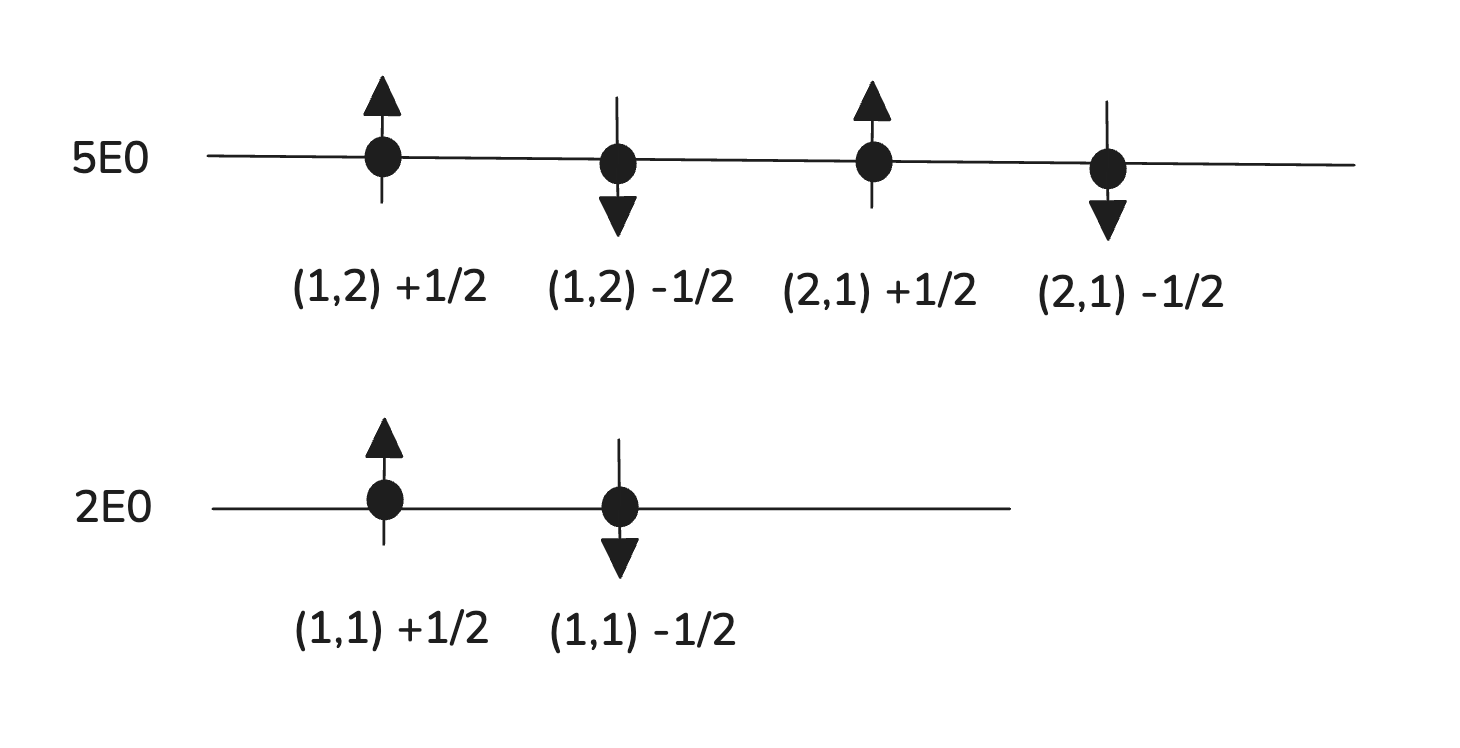
\includegraphics[scale=0.35]{ch10-10.11b.png}
\end{center}
\item [\textbf{(c)}] We can accomodate 10 particles in the box as follows
\begin{center}
    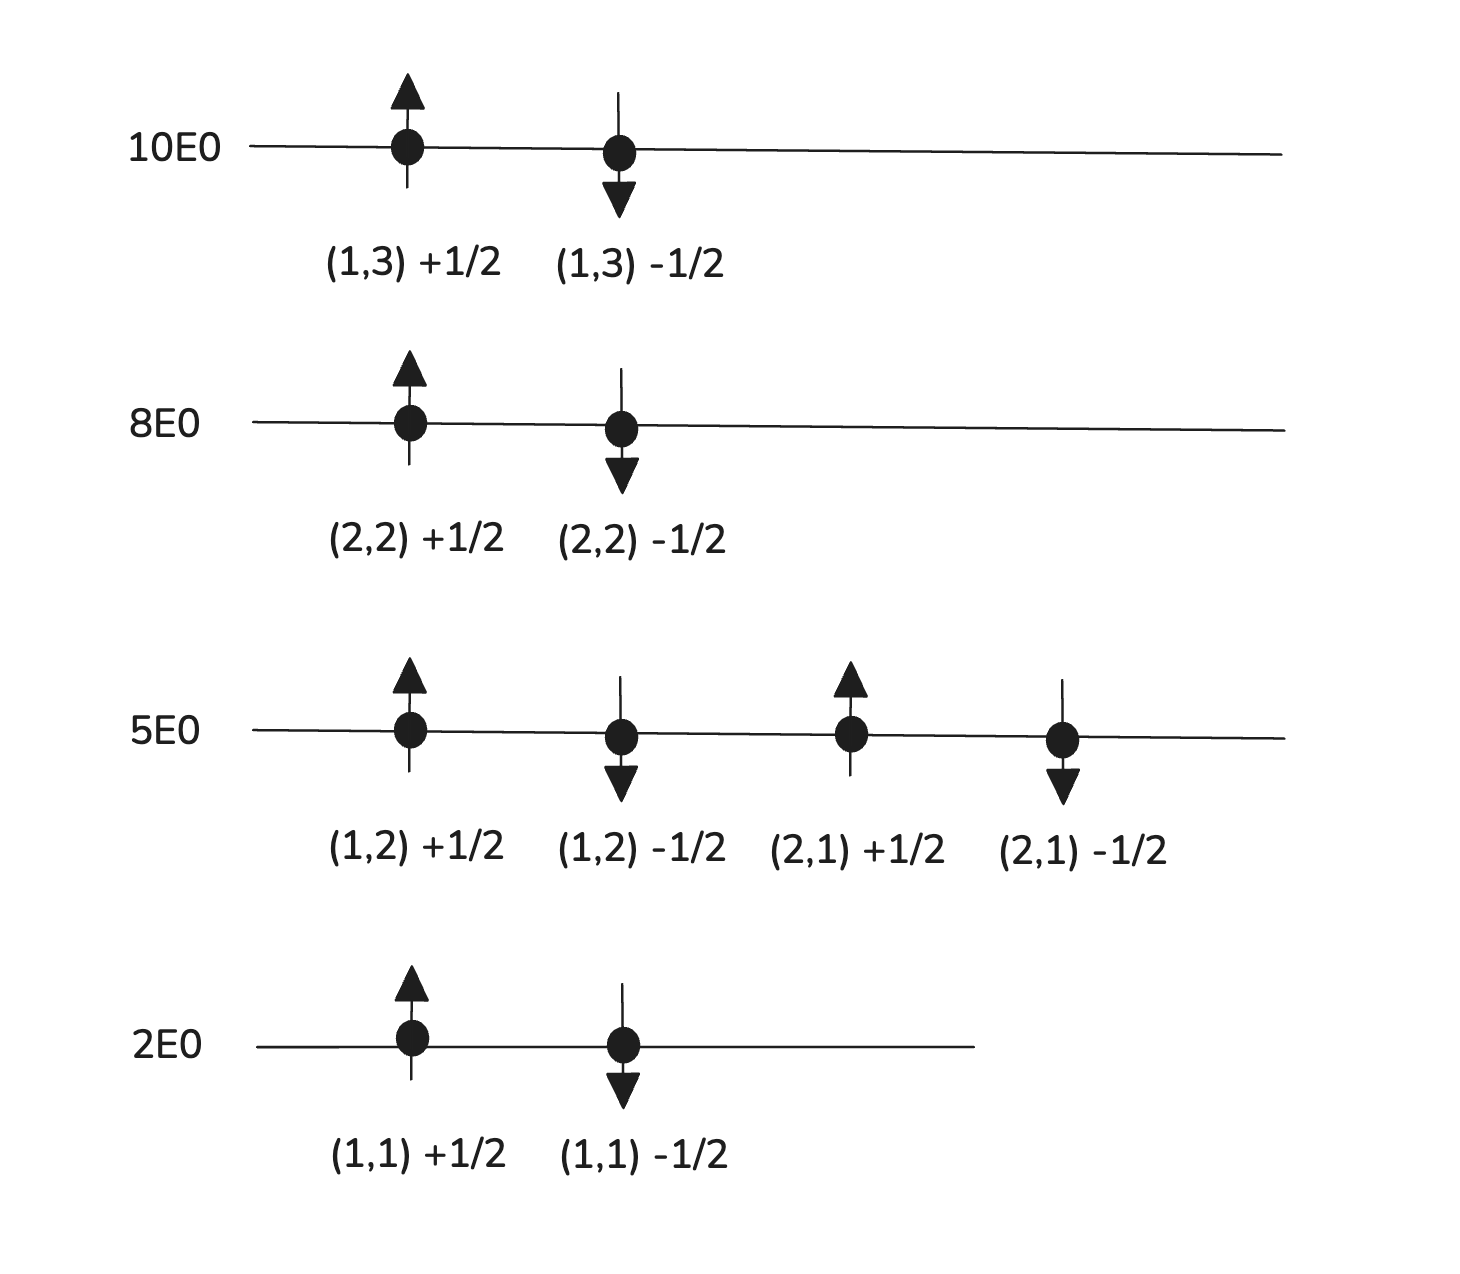
\includegraphics[scale=0.35]{ch10-10.11c.png}
\end{center}

\end{itemize}
\end{proof}

\cleardoublepage
\begin{proof}{\textbf{10.12}}
\begin{itemize}
\item [(a)] Let us consider the wave function
$\psi(x_1, x_2) = e^{-(x_1^2 + x_2^2)}$, we note that
\begin{align*}
    \psi(x_1, x_2) = e^{-(x_1^2 + x_2^2)} = e^{-(x_2^2 + x_1^2)} = \psi(x_2, x_1)
\end{align*}
So the wave function is symmetric. Also, we see that
\begin{align*}
    \int_{-\infty}^\infty \int_{-\infty}^\infty |\psi(x_1,x_2)|^2 ~dx_1 dx_2 = 
    \int_{-\infty}^\infty \int_{-\infty}^\infty e^{-2(x_1^2 + x_2^2)} ~dx_1 dx_2
    = \pi/2
\end{align*}
which implies that the wave function is normalizable.

\item [(b)] Let us consider the wave function
$\psi(x_1, x_2) = x_1 - x_2$, we note that
\begin{align*}
    \psi(x_1, x_2) = x_1 - x_2 = -(x_2 - x_1) = -\psi(x_2, x_1)
\end{align*}
So the wave function is antisymmetric.

\item [(c)] Let us consider the wave function $\psi(x_1, x_2) = 2x_1 - x_2$,
we note that
\begin{align*}
    \psi(x_1, x_2) = 2x_1 - x_2 = -(x_2 - 2x_1) \neq -(2x_2 - x_1) = -\psi(x_2, x_1)
\end{align*}
So the wave function is not antisymmetric, also, let us note that
\begin{align*}
    \psi(x_1, x_2) = 2x_1 - x_2 \neq 2x_2 - x_1 = \psi(x_2, x_1)
\end{align*}
So the wave function is neither symmetric.
\end{itemize}
\end{proof}

\cleardoublepage
\begin{proof}{\textbf{10.13}}
\begin{itemize}
\item [\textbf{(a)}] We know that electrons are fermions so if we have an
electron in the state $(1s, 1/2)$ then the other must be in the state
$(1s, -1/2)$, and since they are indistinguishable swapping them is not
considered as a new atom state, so there is just one independent state of the
whole atom and hence the degeneracy is 1.
\item [\textbf{(b)}] Suppose now that instead of having electrons we have
half-spin bosons then the possible states for the bosons are
\begin{align*}
    (1s, 1/2)~(1s, 1/2)\quad
    (1s, -1/2)~(1s, -1/2)\quad
    (1s, 1/2)~(1s, -1/2)
\end{align*}
Again, since bosons are indistinguishable swapping the last state is not
considered an independent state of the atom, therefore the degeneracy is 3.
\item [\textbf{(c)}] If somehow the two electrons were distinguishable then 
the possible states are
\begin{align*}
    (1s, 1/2)~(1s, 1/2) \qquad
    (1s, -1/2)~(1s, -1/2) \\
    (1s, 1/2)~(1s, -1/2) \qquad
    (1s, -1/2)~(1s, 1/2)
\end{align*}
In this case, we can have the same spin for the two elecrons since they can
be distinguished by their mass. Therefore the degeneracy in this case
is 4.
\end{itemize}
\end{proof}

\cleardoublepage
\begin{proof}{\textbf{10.14}}
For Boron ${}_{5}B$ the energy-level diagram for the ground state looks like
\begin{center}
    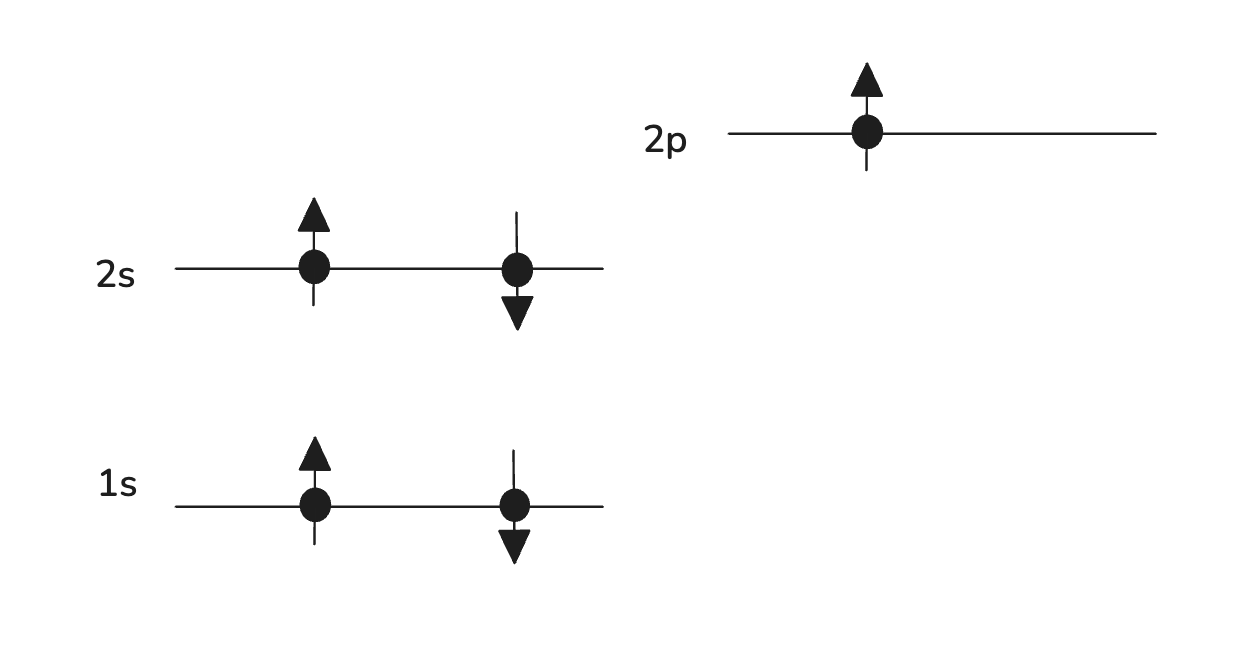
\includegraphics[scale=0.4]{ch10-10.14a.png}
\end{center}
And for the first excited state looks like the following
\begin{center}
    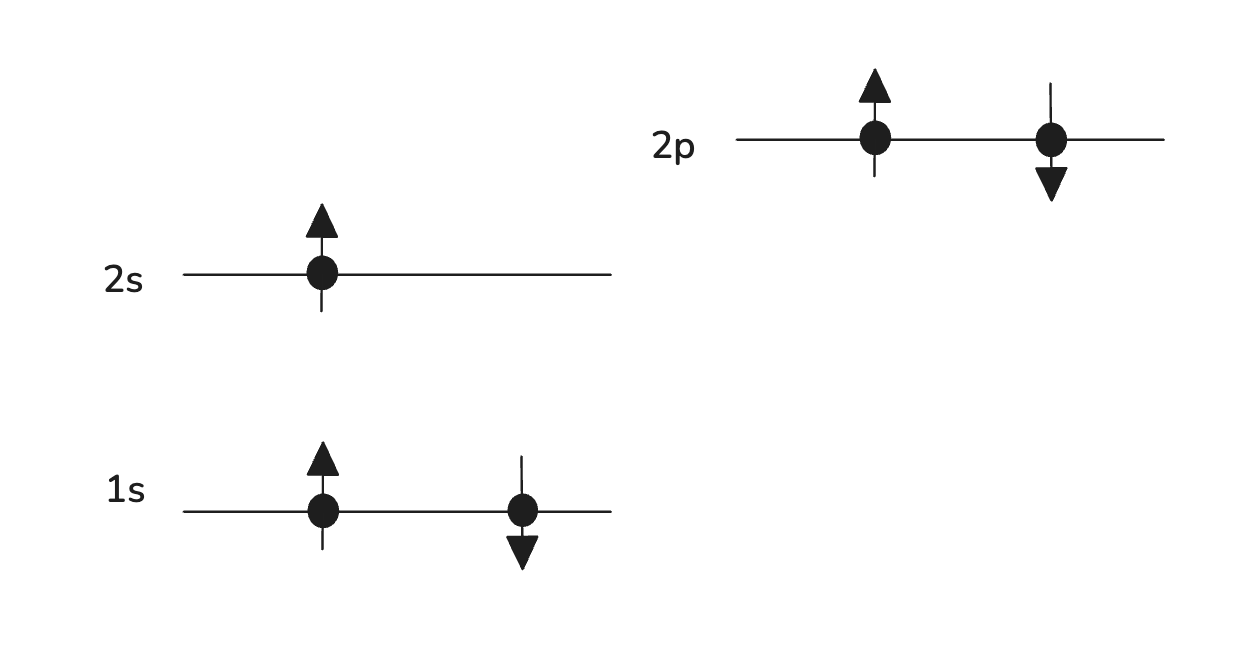
\includegraphics[scale=0.4]{ch10-10.14b.png}
\end{center}
\end{proof}

\cleardoublepage
\begin{proof}{\textbf{10.17}}\\
When jumping from ${}_{4}Be$ to ${}_{5}B$ we have two competing effects:
The increase in $Z$ causes any given level to be somewhat more tightly bound,
but the final electron has to occupy a level that is slightly higher and hence
somewhat less tightly bound.\\
For the ionization energy, the second effect wins, so the ionization energy 
for ${}_{5}B$ is slightly lower than the one for ${}_{4}Be$.
\end{proof}

\cleardoublepage
\begin{proof}{\textbf{10.19}}
\begin{itemize}
\item [\textbf{(a)}] Treating each electron separately as if it were in a
hydrogen-like ion we see that each one has an energy of
\begin{align*}
    E = -Z^2E_R = -4 \cdot 13.6~eV = -54.4~eV
\end{align*}
Therefore in this approximation the total energy of a helium atom is
\begin{align*}
    E_{He} = 2\cdot -54.4~eV = -108.8~eV
\end{align*}
\item [\textbf{(b)}] Assuming both electrons are in the first Bohr orbit with
radius $a_B/2$ on opposite sides of the atom, separated a distance $a_B$ then
the potential energy between the two electrons is
\begin{align*}
    U &= \frac{ke^2}{a_B}\\
    &= \frac{8.9877\sci{9} \cdot (1.602\sci{-19})^2}{5.29\sci{-11}}\\
    &= 4.3603\sci{-18}~J = 27.214~eV
\end{align*}
Therefore the total energy of a helium atom adding the potential energy between
the electrons is
\begin{align*}
    E_{He} = -108.8 + 27.214 = -81.586~eV
\end{align*}
This is a close approximation to the measured value of $-79.0~eV$. 
\end{itemize}
\end{proof}

\cleardoublepage
\begin{proof}{\textbf{10.23}}\\
We see that $Cd$ ($Z = 48$) has it's $4d$ level full and hence $In$ ($Z = 49$) 
has 1 electron at the level $5p$, so $In$ has an electron in a level
with higher energy and hence it's less tightly bound, so the ionization
energy has a drop.\\
In the same way, $Hg$ ($Z = 80$) has from the 6th shell the levels $4f$, $5d$ 
and $6s$ full of electrons. They are filled in that order since, for example,
$4f$ has lower energy than $5d$. Then $Tl$ ($Z = 81$) has 1 electron at the 
next sub-shell $6p$ which has higher energy and hence is less tightly bound,
therefore the ionization energy has a drop. 
\end{proof}

\cleardoublepage
\begin{proof}{\textbf{10.27}}\\
If the electron had a spin $s = 3/2$ then there are 4 possible spins
$-3/2, -1/2, 1/2$ and $3/2$ so the $s$ level can have 4 electrons, the $p$
level can have 12 electrons and the $d$ level can have 20 electrons.\\
Then the ground-state configurations for ${}_{8}O$, ${}_{10}Ne$ and ${}_{21}Sc$
are
\begin{align*}
    {}_{8}O&:\quad 1s^4 2s^4\\
    {}_{10}Ne&:\quad 1s^4 2s^4 2p^2\\
    {}_{21}Sc&:\quad 1s^4 2s^4 2p^{12} 3s^1
\end{align*}
\end{proof}

\cleardoublepage
\begin{proof}{\textbf{10.33}}\\
\begin{itemize}
\item [(a)] Assuming the ionization energies vary linearly from ${}_{20}Ca$
to ${}_{38}Sr$ then the slope of the linear interpolation formula is
\begin{align*}
    m = \frac{5.70 -6.11}{38 - 20} = -0.0227
\end{align*}
So for ${}_{56}Ba$ we have that
\begin{align*}
    y = y_1 + m(x - x_1) = 6.11 - 0.0227(56 - 20) = 5.292~eV
\end{align*}
This value is close to the observed value of $5.21~eV$.
\item [(b)] Assuming the electron affinity vary linearly from ${}_{17}Cl$
to ${}_{53}I$ then the slope of the linear interpolation formula is
\begin{align*}
    m = \frac{3.06 - 3.61}{53 - 17} = -0.01527
\end{align*}
So for ${}_{35}Br$ we have that
\begin{align*}
    y = y_1 + m(x - x_1) = 3.61 - 0.01527(35 - 17) = 3.335~eV
\end{align*}
\item [(c)] Assuming the atomic radius vary linearly from ${}_{7}N$
to ${}_{8}O$ then the slope of the linear interpolation formula is
\begin{align*}
    m = \frac{0.065 - 0.075}{8 - 7} = -0.01
\end{align*}
So for ${}_{9}F$ we have that
\begin{align*}
    y = y_1 + m(x - x_1) = 0.075 - 0.01(9 - 7) = 0.055~nm
\end{align*}

\end{itemize}
\end{proof}

\cleardoublepage
\begin{proof}{\textbf{10.35}}\\
Assuming the electron affinity vary linearly from ${}_{17}Cl$
to ${}_{35}Br$ then the slope of the linear interpolation formula is
\begin{align*}
    m = \frac{3.36 - 3.62}{35 - 17} = -0.014
\end{align*}
So for ${}_{9}F$ we have that
\begin{align*}
    y = y_1 + m(x - x_1) = 3.62 - 0.014(9 - 17) = 3.73~eV
\end{align*}
Which is not that close to the observed value of 3.40 eV.
\end{proof}

\cleardoublepage
\begin{proof}{\textbf{10.36}}\\
The energy of the $1s$ electrons is approximately $Z^2 E_R = -122.4~eV$
for the lithium atom.
Comparing this value to the ones in figure 10.16 we see that the lowest
five excited levels must be
\begin{align*}
    1s^2 2p^1 \qquad
    1s^2 3s^1 \qquad
    1s^2 3p^1 \qquad
    1s^2 3d^1 \qquad
    1s^2 4s^1
\end{align*}
Since it requires less energy to move the $2s$ electron to a higher level
compared to the $1s$ electrons.
\end{proof}

\cleardoublepage
\begin{proof}{\textbf{10.40}}\\
The potential energy $U(r)$ associated to $\mathscr{E}$ is given by 
\begin{align*}
    U(r) &= -\int (-e)\mathscr{E} ~dr\\
    &= e^2k\int \frac{1}{r^2}
    \bigg[1 + \frac{(Z-1)}{2 R^2}e^{-r/R}(r^2 + 2rR + 2R^2)\bigg] ~dr\\
    &= e^2k\int \frac{1}{r^2}
    + \frac{(Z-1)}{2 R^2}
    \bigg(e^{-r/R} + \frac{2Re^{-r/R}}{r} + \frac{2R^2e^{-r/R}}{r^2}\bigg) ~dr\\
    &= e^2k\int \frac{1}{r^2}
    + \frac{(Z-1)}{2 R^2}
    \bigg(e^{-r/R} + \frac{2Re^{-r/R}}{r} + \frac{2R^2e^{-r/R}}{r^2}\bigg) ~dr\\
    &= e^2k\bigg[ -\frac{1}{r}
    + \frac{(Z-1)}{2 R^2}
    \bigg(-Re^{-r/R} + 2R \text{Ei}(-r/R) - 2R \text{Ei}(-r/R) - \frac{e^{-r/R}}{r}\bigg)\bigg]\\
    &= -e^2k\bigg[ \frac{1}{r}
    + \frac{(Z-1)}{2 R^2}
    e^{-r/R}\bigg(R + \frac{1}{r}\bigg)\bigg]
\end{align*}
Ploting this equation and equations (10.4) and (10.5) we see that
\begin{center}
    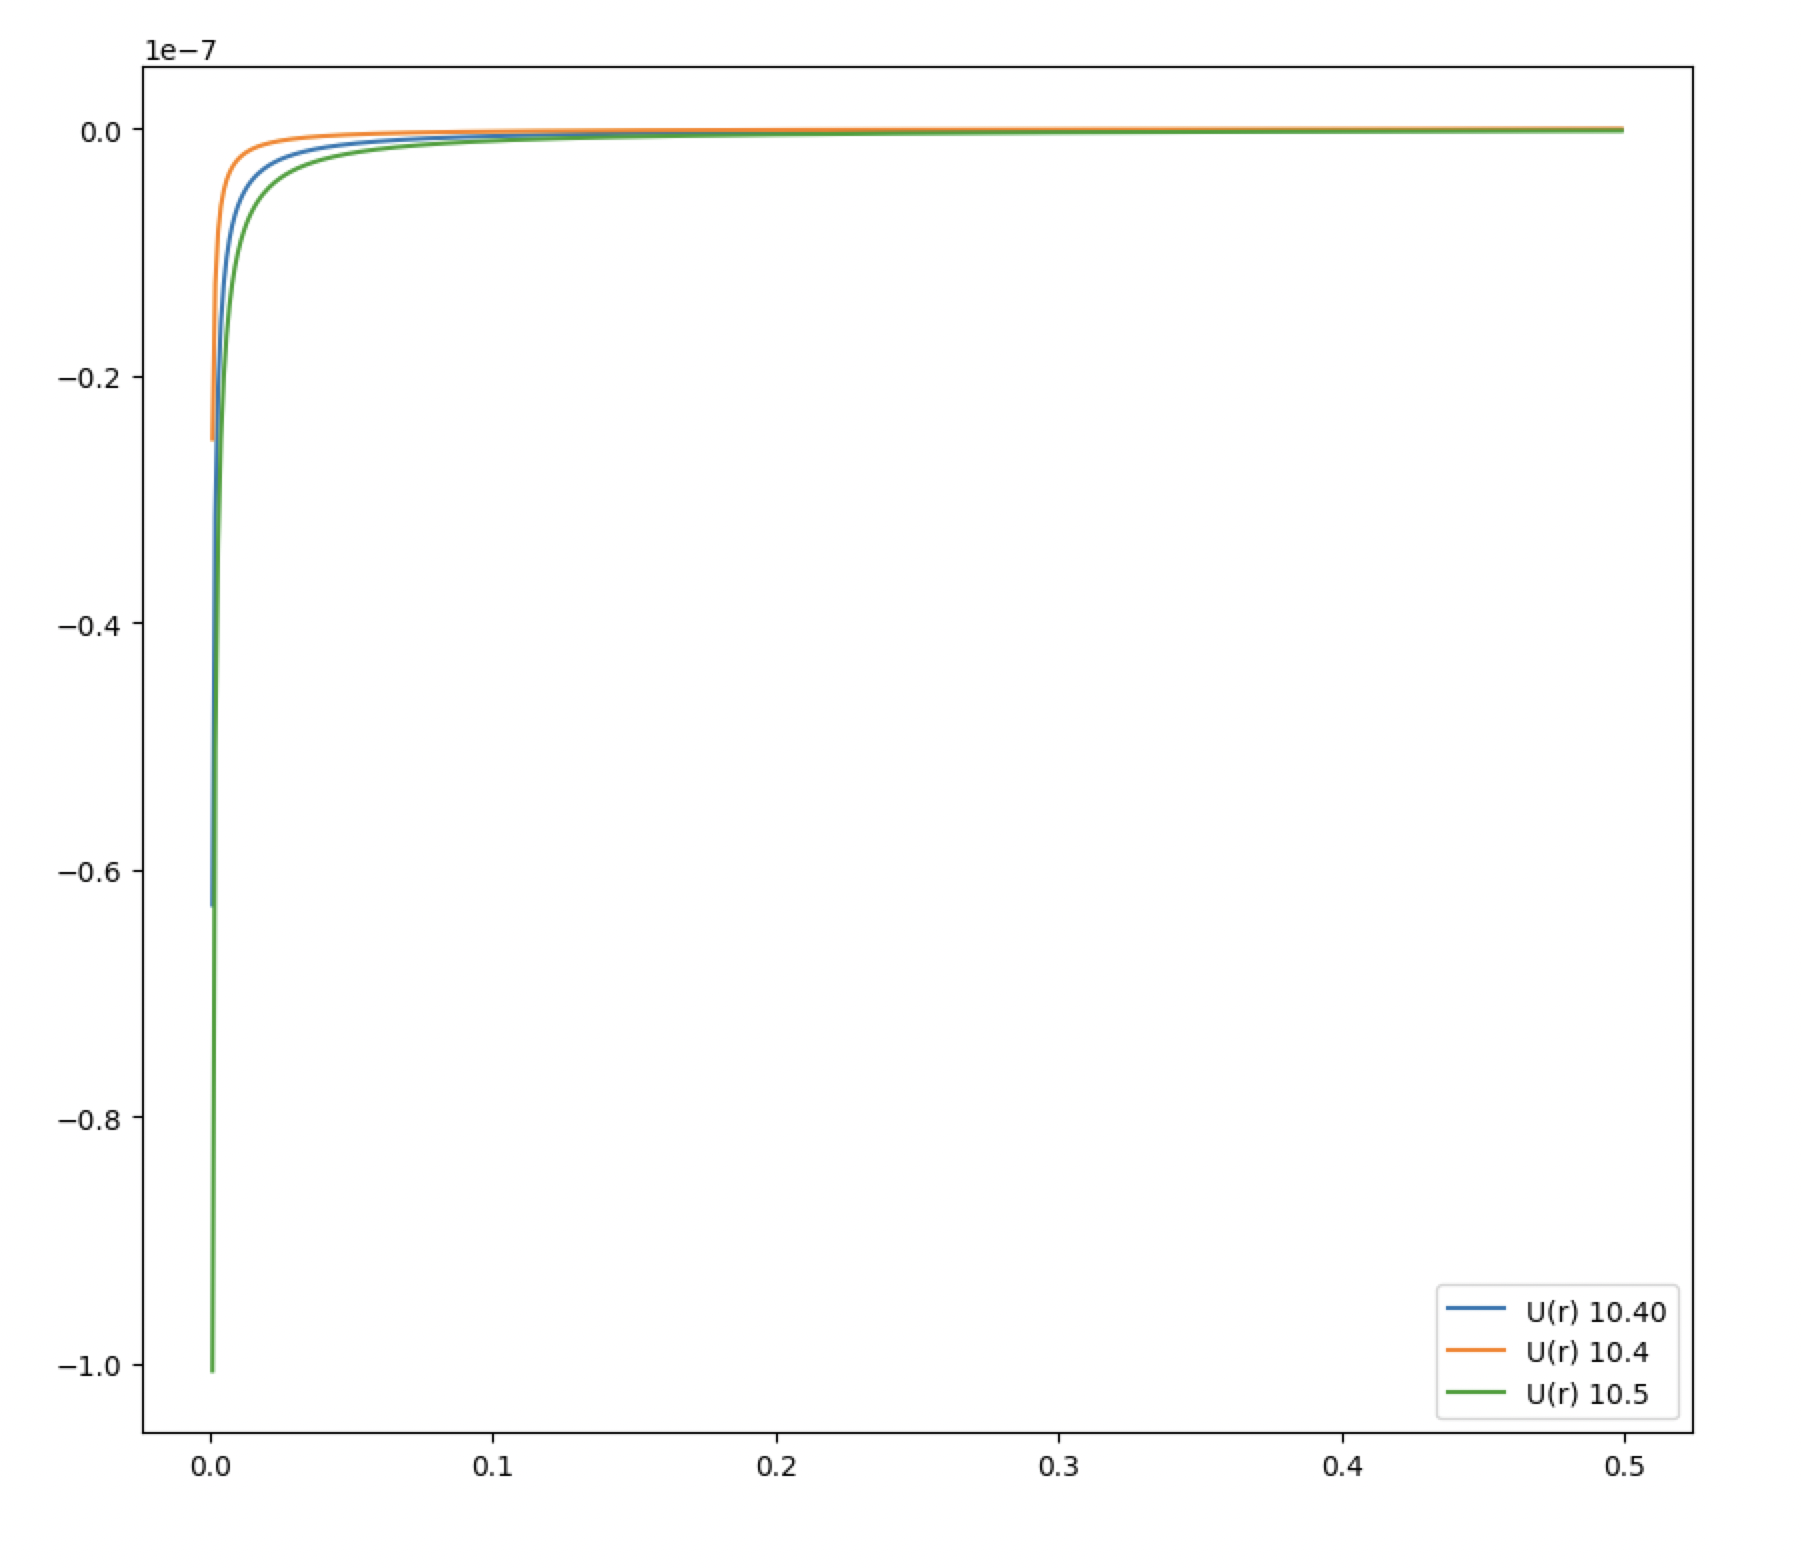
\includegraphics[scale=0.45]{ch10-10.40.png}
\end{center}
\end{proof}
\end{document}